\documentclass[serif,professionalfonts]{beamer}

\usetheme{Forcellini}

\usepackage{amsmath}
\usepackage{amssymb}
\usepackage{amsthm}

% Hermann Zapf Optima clone (wonderful sanserif font) -- URW Classico
\renewcommand{\sfdefault}{uop}
\renewcommand{\rmdefault}{ppl}

\usepackage{fixltx2e}
\usepackage{microtype}

\usepackage{dot2texi}
\usepackage{readarray}
\usepackage{tikz}
\usetikzlibrary{calc} %for calculations in tikz commands
\usetikzlibrary{positioning}
\usetikzlibrary{arrows}
\usepackage{tikz-qtree}
\usepackage{xxcolor}

\setbeamertemplate{navigation symbols}{}
\usepackage{hyperref}
\usepackage[utf8]{inputenc}
\usepackage[T1]{fontenc}

\usepackage{comment}
% description with short indentation
\setbeamersize{description width of=x}

\setbeamertemplate{caption}
{
  \raggedright%
  \insertcaption\par%
}
\setbeamercolor{green}{fg=green}

\newcommand\todo[1]{\textcolor{red}{(TODO: #1)}}
\newcommand\load{L_{\mathrm{max}}}
\newcommand\loadS{\load^{\mathrm{S}}}
\newcommand\loadG{\load^{\mathrm{G}}}
\newcommand\loadAgl{\load^{\mathrm{A}}}
\newtheorem{claim}{Claim}
\newtheorem{assumption}{Assumption}
\newtheorem{invariant}{Invariant}

\newcommand\xqed[1]{%
   \rlap{\hbox to#1{\hfil\llap{\ensuremath{\qed}}}}
}

%---------------------------------------------------------------------
% Create Color definition From Template
%---------------------------------------------------------------------
% #1 template name, 
% #2 foreground color name
% #3 background color name
\newcommand{\ccft}[3]{
\usebeamercolor{#1}
\definecolor{#2}{named}{fg}
\definecolor{#3}{named}{bg}
}
%get some colors from the scheme
\ccft{block body example}{examplefg}{examplebg} 

%---------------------------------------------------------------------
%parameters for balls into bins graphs
%---------------------------------------------------------------------
%scale factor
\newcommand\scalefac{0.55}
%diameter of balls
\newcommand\ballsize{5mm}
%number of bins
\newcommand\nrbins{6}
%space between ball and bin
\newcommand\padding{0.1*\ballsize}
%height of a bin
\newcommand\binheight{5*\balldiameter}
%width of a bin
\newcommand\binwidth{\balldiameter}
%gap from bin to bin
\newcommand\bingap{1.6*\balldiameter}
%color of balls
\tikzstyle{ballstyle} = [ball color=black!30!red]
\tikzstyle{specialBallstyle} = [ball color=black!30!red,  opacity=0.2]

%---------------------------------------------------------------------
%tikz styles and commands
%---------------------------------------------------------------------
\newcommand\balldiameter{2*\ballsize}

%arrow style
\tikzstyle{insert} = [
	thick,->,>=stealth'
]

%draw an arrow symbolizing a location
\newcommand\iA[2][0]{
	\path (\nbid) edge[insert, bend left=#1] (#2);
}
%bin style
\tikzstyle{topflat} = [
	minimum width=(\binwidth+2*\padding)*\scalefac, 
	minimum height=(\binheight+4*\padding)*\scalefac,
	append after command={
    		\pgfextra
        		\fill[fill=examplebg] 
        			(\tikzlastnode.north east) [rounded corners] |-
        			(\tikzlastnode.south)  -| 
        			(\tikzlastnode.west) [sharp corners] |- 
        			(\tikzlastnode.north) -- cycle;
	         \draw[rounded corners] 
	         	(\tikzlastnode.north east) |- 
	         	(\tikzlastnode.south) -| 
	         	(\tikzlastnode.north west);
    		\endpgfextra
    }
]    

%draw i'th bin
\newcommand\bin[1]{
	\path node[topflat, xshift=#1*\bingap*\scalefac, above, yshift=-\padding*\scalefac]  {};
}

%draw all bins
\newcommand\bins{
	\foreach \ibin in {1,...,\nrbins}
		\bin{\ibin};
}

%set a node at bin #1, position #2 with node id = #1+(#2-1)*6
\newcommand\setNode[2]{
	\draw let \n1 ={#1#2} in node[circle, minimum size = \ballsize](n\n1) at (#1*\bingap,#2*\balldiameter-\ballsize) {};
}

%create nodes for all possible balls
\newcommand\nodes{
	\foreach \i in {1,...,6}
		\foreach \j in {1,...,5}
			\setNode{\i}{\j};
}

%paint a ball in bin #1, position #2 with style specialBallstyle
\newcommand\specialBall[2]{
	\shade[specialBallstyle] (#1*\bingap,#2*\balldiameter-\ballsize) circle (\ballsize) {};
}

%paint a ball in bin #1, position #2 with style = ballstyle
\newcommand\ball[2]{
	\shade[ballstyle] (#1*\bingap,#2*\balldiameter-\ballsize) circle (\ballsize) {};
}

%paint a ball that is to be inserted
\newcommand\nbid{nb}
\newcommand\newball{
	\draw node[circle, minimum size = \ballsize](\nbid) at (0*\bingap,6*\balldiameter-\ballsize) {};
	\ball{0}{6};
}

%put #2 balls into bin 1 <= #1 <= 6
\newcommand\putinbin[2]{
	\ifnum #2 > 0
		\foreach \nrballs in {1,...,#2}
 			\ball{#1}{\nrballs};
 	\fi
}

%put balls into bins. #i: number of balls to put in i'th bin
\newcounter{index}
\newcommand\balls[1]{%
	\getargsC{#1}%
  	\setcounter{index}{0}%
  	\whiledo{\theindex < \narg}{%
    		\stepcounter{index}%
    		\putinbin{\theindex}{\csname arg\romannumeral\theindex\endcsname}%
  	}%
}

%draw balls and bins. #i: number of balls to put in i'th bin
\newcommand\bab[1]{%
	\bins
	\nodes
	\balls{#1}
}
%draw group seperator after bin #1
\newcommand\groupSep[1]{
	\draw[thick, color=red!40] let \n1={(#1+0.5)*\bingap} in (\n1,-\ballsize) -- (\n1,\binheight +\ballsize);
}

%---------------------------------------------------------------------
% tikz stuff
%---------------------------------------------------------------------

% nicer tikz qtrees
\tikzset{edge from parent/.style=
     {draw, edge from parent path={(\tikzparentnode) -- (\tikzchildnode)}}}
\tikzset{every tree node/.style={font=\tiny, thick, align=center}}    
     
%---------------------------------------------------------------------
%Front matter
%---------------------------------------------------------------------
\title{The Power of Two Random Choices}
\subtitle{\dots and the Surprising Influence of Asymmetry}
\author[M. Kalany]{Martin Kalany}
\institute[TU Wien]
{
  Graduate student in Computer Science\\
  Vienna University of Technology\\
}
\date{\today}

%---------------------------------------------------------------------
%document
%---------------------------------------------------------------------
% Structure:
% 30 min
% 5 min easy stuff (so that everyone understands)
% 5 min more advanced stuff 
% 15 min difficult stuff (the proof, of the asymmetric allocation scheme using the infamous assumption 1)
% 5 min further results and wrap up
\begin{document}
\begin{frame}
  \titlepage
\end{frame}

\begin{frame}
\frametitle{The problem}
\framesubtitle{...and the goal}
\begin{exampleblock}{Balls-into-bins games}
Suppose we have $n$ initially empty bins and need to distribute $m \geq n$ balls among them, \alert{as evenly as possible}. 
\end{exampleblock}
\pause
\begin{exampleblock}{Definition}
We are interested in the \alert{maximum load $\load$}, i.e, how many balls are in the fullest bin?
\end{exampleblock}

\begin{exampleblock}{Definition}
Equivalently, we can look at the \alert{additive gap} $\delta$:
\begin{align*}
\delta = \load - \frac{m}{n}
\end{align*}
\end{exampleblock}
\end{frame}

\begin{frame}
\frametitle{Single choice strategy}
\framesubtitle{A basic allocation scheme}
\begin{exampleblock}{Basic idea}
For each ball, choose one of the $n$ bins \alert{uniformly and independently at random}.
\end{exampleblock}
\bigskip

\begin{center}
\begin{tikzpicture}[scale=\scalefac]
	\bab{2 1 4 2 3 0}
	\newball
	\iA[40]{n23};
\end{tikzpicture}
\end{center}
\end{frame}

\begin{frame}
\frametitle{Single choice strategy}
\framesubtitle{Upper bound for the maximum load}
%&Since we deal with a \alert{random process}, we cannot give upper bounds for the maximum load $\load$ with absolute certainty! 

\begin{exampleblock}{Definition}
We say that an event $\mathcal E_n$ occurs \alert{with high probability} (w.h.p.) if $\Pr\left[\mathcal E_n \right] \geq 1 - n^{-\alpha}$ for some $\alpha > 0$.
\end{exampleblock}

\pause
\medskip
We distinguish the \alert{lightly loaded} case ($m = n$) and the \alert{heavily loaded} case ($m \in \omega(n\ln n)$).

\medskip
\begin{theorem}[Raab and Steger, 1998]
When using the \alert{single choice} strategy to distribute $m$ balls to $n$ bins, the maximum load will be, w.h.p.,
\begin{align*}
\loadS \leq 
	\begin{cases}
    \Theta\left(\frac{\ln n}{\ln\ln n}\right)           & m = n \\
    \frac{m}{n} + \Theta\left(\sqrt{\frac{m\ln n}{n}} \right)              & m \in \omega(n \ln n)
    \end{cases} \quad .
\end{align*}
\end{theorem}
\end{frame}

\begin{frame}
\frametitle{Multiple choice strategies}
\begin{exampleblock}{Idea}
Put a ball into the \alert{least full} of $d\geq2$ randomly chosen bins.
\end{exampleblock}

\bigskip
We distinguish placement algorithms by the way the $d$ \alert{bins are sampled}:
\begin{enumerate}
\item Uniformly and independently
\item Non-uniformly and independently
\item Non-uniformly and dependently
\end{enumerate}
\end{frame}

\begin{frame}
\frametitle{The Greedy algorithm}
\begin{exampleblock}{Algorithm}
\begin{enumerate}
\item For each ball, choose $d$ bins independently and uniformly at random. 
\item Put the ball into the least full bin.
\item In case a tie occurs, choose one of the $d$ bins arbitrarily.
\end{enumerate}
\end{exampleblock}

\only<1>{
\begin{center}
\begin{tikzpicture}[scale=\scalefac]
	\bab{2 1 4 2 3 0}
	\newball
	\iA[35]{n22};
	\iA[35]{n44};
\end{tikzpicture}
\end{center}
}

\only<2->{
\begin{theorem}[Azar, Broder, Karlin and Upfal, 1999]
When using the \alert{Greedy} algorithm to distribute $m$ balls to $n$ bins, the maximum load will be, w.h.p.,
\begin{align*}
\loadG \leq \frac{m}{n} + \frac{\ln \ln n}{\ln d} + O(1) \quad .
\end{align*}
\end{theorem}
}
\end{frame}

\begin{frame}
\frametitle{Single choice vs.~Greedy}
\begin{align*}
\loadS \leq 
	\begin{cases}
    \Theta\left(\frac{\ln n}{\ln\ln n}\right)           & m = n \\
    \frac{m}{n} + \Theta\left(\sqrt{\frac{m\ln n}{n}} \right)              & m \in \omega(n \ln n)
    \end{cases}
\end{align*}
\begin{align*}
\loadG \leq \frac{m}{n} + \frac{\ln \ln n}{\ln d} + O(1) 
\end{align*}

\begin{alertblock}{The two-choice paradigm}
Even for $d=2$, Greedy achieves an \alert{exponential decrease} of the additive gap $\delta$, which does \alert{not depend on} the number of balls \alert{$m$}.
\end{alertblock}
\end{frame}

\begin{frame}
\frametitle{Applications}
\begin{description}
	\item[Hashing:] Assuming a perfect hash function, $n$ elements (balls) are mapped to $m$ table entries (bins). Using two hash functions: look-up time $\Theta(\ln\ln n)$, w.h.p. \alert{Easy to parallelize} and  \alert{no re-hashing}!
	\item[Online load balancing:] Assign tasks (balls) to servers/processors (bins). The two-choice paradigm helps to \alert{reduce communication overhead}, %(of e.g., a central dispatcher)
	while the maximum load will be $\Theta(\ln\ln n)$, w.h.p.
	\item[Emulating PRAMs on DMMs:] Distribute processors and memory cells of the PRAM on the DMM s.t.~the overhead of the emulation is minimized.
	\item[Low congestion circuit routing:] \alert{Valiant's paradigm} %(a permuation routing problem can be split into two sub-problems: route to random intermediate destination and then on to the actual destination) 
	is analogous to the single-choice technique.
\end{description}
\end{frame}


\newcommand\aglAlgorithm{
\begin{exampleblock}{Algorithm}
\begin{enumerate}
\item Partition the $n$ bins into $d$ groups.
\item Assume a fixed ordering of the bins $b_i$, $1\leq i \leq n$.
\item Choose one bin from each group uniformly and independently.
\item Put the ball into the least full bin.
\item In case a tie occurs, put the ball into the leftmost bin (i.e., the bin with smallest index) among those with same minimal load.
\end{enumerate}
\end{exampleblock}
}

\begin{frame}[shrink]
\frametitle{The Always-go-left algorithm}
\aglAlgorithm

\begin{center}
\begin{tikzpicture}[scale=\scalefac]
	\bab{2 1 4 2 3 0}
	\newball
	\groupSep{3};
	\iA[30]{n13};
	\iA[30]{n54};	
\end{tikzpicture}
\end{center}

\end{frame}

\begin{frame}
\frametitle{$d$-step Fibonacci numbers and the golden ratio}
\framesubtitle{(Capocelli, Cull, 1990)}

$d$-step Fibonacci numbers:
\begin{align*}
F_d(k) := \begin{cases}
                0               & k \leq 0\\
                1               & k = 1\\
                \sum_{i=1}^{d}F_d(k-i) & k > 1
            \end{cases}
\end{align*}
Generalized golden ratio $\Phi_d$:
\begin{align*}
\Phi_d := \lim_{k \rightarrow \infty} \frac{F_d(k)}{F_d(k-1)}
\end{align*}
\begin{align*}
\Phi_2 = 1.61 \quad , \quad \forall i\; \forall j \in \mathbb{N}: i < j \implies \Phi_i < \Phi_j \quad , \quad \lim_{d\rightarrow \infty} \Phi_d = 2 
\end{align*}
\begin{align*}
F_d(k) \geq \Phi_d^{k-2}
\end{align*}
\end{frame}

\newcommand\theoremVocking{
\begin{theorem}[V\"ocking, 2003]
When using the \alert{Always-go-left} algorithm to distribute $m$ balls to $n$ bins, the maximum load will be, w.h.p.,
\begin{align*}
\loadAgl \leq \frac{m}{n} + \frac{\ln \ln n}{d \ln \Phi_d} + O(1) \quad .
\end{align*}
\end{theorem}
}

\begin{frame}[shrink]
\frametitle{The Always-go-left algorithm}
\aglAlgorithm
\theoremVocking
\end{frame}

\begin{frame}
\frametitle{The Always-go-left algorithm}
\begin{columns}[onlytextwidth]
\begin{column}{0.5\textwidth}
\begin{align*}
\loadG \leq \frac{m}{n} + \frac{\ln \ln n}{\ln d} + O(1) 
\end{align*}
\end{column}
\begin{column}{0.5\textwidth}
\begin{align*}
\loadAgl \leq \frac{m}{n} + \frac{\ln \ln n}{d \ln \Phi_d} + O(1)
\end{align*}
\end{column}
\end{columns}
\bigskip
The combination of \alert{asymmetric tie breaking} and \alert{non-uniform} (and independent) sampling of the $d$ bins is crucial to achieve this upper bound.
\bigskip
\begin{theorem}[V\"ocking, 2003]
For $m=n$, using an arbitrary allocation scheme that chooses $d$ bins for each ball at random (i.e., class 3), the maximum load is, w.h.p,
\begin{align*}
\loadAgl = \frac{\ln \ln n}{d \ln \Phi_d} - O(1) \quad .
\end{align*}
\end{theorem}
\end{frame}

\begin{frame}
\frametitle{BiB Model}
We will assume a sequential, infinite, dynamic process.

\begin{description}
\item[Sequential:] The balls arrive one after another, one at each time step~$t$.
\item[Infinite:] Ball placements and deletions are given for an infinite time span.
\item[Dynamic:] Balls do not stay in the bins forever.
\begin{itemize}
\item An oblivious adversary provides a sequence $\sigma = \sigma_1 \sigma_2 \dots$, where $\sigma_t = (d_t, a_t)$.
\item $d_t$/$a_t$: ball to delete/add at time step t. \\
\item $\sigma$ is fixed in advance.
\end{itemize}
\end{description}
\end{frame}

\begin{frame}
\frametitle{The Always-go-left algorithm}
\framesubtitle{Proof of the upper bound for $m=n$}
\begin{theorem}[V\"ocking, 2003]
\label{theorem:aglm}
Consider any sequence of insertions and deletions s.t.~at most $n$ balls are in the bins at any time. If the balls are placed into bins by the Always-go-left algorithm, the maximum load at any time step $t$ is, w.h.p., 
\begin{align*}
\loadAgl \leq \frac{\ln\ln n}{d  \ln \Phi_d} + O(1) \quad .
\end{align*}
\end{theorem}

\pause
\bigskip
In case $\load$ exceeds a given threshold of $L+3$ balls ("a bad event occurs"), we construct an activated \alert{witness tree of order $L$}. The probability for its existence upper bounds the probability that the associated bad event occurs.  
\end{frame}

\newcommand\assumptionOne{
\begin{alertblock}{Assumption}
All the events represented by the nodes and edges of a witness tree are stochastically independent. 
\end{alertblock}
}

\begin{frame}
\frametitle{Witness trees}
A witness tree
\begin{itemize}
\item is a \alert{tree-like structure},
\item where each node $v$ references a ball $b_v$ and
\item nodes and edges represent \alert{events} (that may occur or not),
\item that are, in general, \alert{not independent}.
\item It is \alert{activated} when all its leaf and edge events occur. 
\end{itemize}

\bigskip
\assumptionOne
\end{frame}

\begin{frame}
\frametitle{Asymmetric witness trees (AWT)} 
A $d$-ary AWT of order $L$ has the structure of a Fibonacci tree $T_d(dL+1)$:

\begin{center}
\begin{tikzpicture}[scale=1]
 \Tree 
 	[.$T_d(7)$ \edge[draw, dotted];
		[.$T_d(6)$
			[.$T_d(5)$
				[.$T_d(4)$ 
					[.$T_d(3)$ $T_d(2)$ $T_d(1)$ ]
					$T_d(2)$ %$T_d(1)$
				]
				[.$T_d(3)$ $T_d(2)$ $T_d(1)$ ]
				%$T_d(2)$
			]
			[.$T_d(4)$ 
				[.$T_d(3)$ $T_d(2)$ $T_d(1)$ ]
				$T_d(2)$ %$T_d(1)$
			]
			%[.$T_d(3)$ $T_d(2)$ $T_d(1)$ ]
		]
		\edge[draw=none]; {}
		%\edge[draw=none]; {}		
	]
\end{tikzpicture}
\end{center}
\end{frame}

\newcommand\defEdgeEvent{
\begin{exampleblock}{Edge event}
Edge $e =(u,v)$, s.t.~$v$ is $i$-th child of $u$: $e$ represents the event that the $i$-th location of ball $b_u$ points to the same bin as one of the locations of ball $b_v$.
\end{exampleblock}
}

\newcommand\defLeafEvent{
\begin{exampleblock}{Leaf event}
A leaf node $v$ represents the event that each of the $d$ locations of the ball $b_v$ points to a bin that contains at least three additional balls, at the time of the insertion of the ball $b_v$.
\end{exampleblock}
}

\begin{frame}
\frametitle{Edge events}
\defEdgeEvent
\begin{center}
\begin{tikzpicture}[every tree node/.style={thick}]
 \Tree 
 	[.\node[draw,circle]{u}; 
		\edge[draw, densely dotted]; {}  
		%\edge[draw, densely dotted]; {}
		\edge[draw] node[draw=none, thick, anchor=west] {$i$};
		[.\node[draw,circle]{v};
		]
	]
	\node (bu) at (0.75,0.5) {};
	\node (bv) at (1.1,-1.25) {};
	
	\path node[topflat, xshift=3.5cm, above, yshift=-3cm]  {};
	\node[circle] (bin1) at (3.5,-0.75) {};
	
	\path node[topflat, xshift=4.5cm, above, yshift=-3cm]  {};
	\node[circle] (bin2) at (4.5,-0.75) {};
	
	\path node[topflat, xshift=5.5cm, above, yshift=-3cm]  {};
	\node[circle] (bin3) at (5.5,-0.75) {};
	
	\path node[topflat, xshift=6.5cm, above, yshift=-3cm]  {};
	\node[circle] (bin4) at (6.5,-0.75) {};
	
	\path node[topflat, xshift=7.5cm, above, yshift=-3cm]  {};
	\node[circle] (bin5) at (7.5,-0.75) {};
	
	\path node[topflat, xshift=8.5cm, above, yshift=-3cm]  {};
	\node[circle] (bin6) at (8.5,-0.75) {};
	
	\path (bu) edge[insert, bend left=20] node[draw=none, font=\tiny, sloped, anchor=south]{$i$-th location} (bin3);
	\path (bu) edge[insert, dotted, bend left=30] (bin6);
	
	\path (bv) edge[insert, bend right=30] node[draw=none, font=\tiny, sloped, anchor=south]{any location} (bin3);
	\path (bv) edge[insert, dotted, bend right=40] (bin4);
	
	\shade[ballstyle] (0.75,0.5) circle (\ballsize*\scalefac) {};
	\shade[ballstyle] (1.1,-1.25) circle (\ballsize*\scalefac) {};
\end{tikzpicture}
\end{center}
\end{frame}

\begin{frame}
\frametitle{Leaf events}
\defLeafEvent

\bigskip
\begin{center}
\begin{tikzpicture}[every tree node/.style={thick}]
\begin{scope}[xshift=-0.9cm, yshift=4cm]
\Tree
 	[.\node[draw,circle]{u}; 
		\edge[draw, densely dotted]; {}  
		\edge[draw] {};
		[.\node[draw,circle]{v};
		]
	]
\end{scope}
\begin{tikzpicture}[scale=\scalefac]
\begin{scope}[yshift=1cm]
	\bab{3 0 0 0 3 0}
	\newball
	\iA[30]{n14};
	\iA[25]{n54};	
\end{scope}
\end{tikzpicture}

\end{tikzpicture}
\end{center}


\end{frame}

\begin{frame}[shrink]
\frametitle{Asymmetric witness trees (AWT)} 
We assign a label $(h,i)$, with $0\leq h \leq L$, $1\leq i \leq d$, to each node:
\begin{itemize}
\item Node $T_d(1)$/$T_d(2)$ is labeled $(0,1)$/$(0,2)$.
\item For $i>2$, a node $(0,i)$ has $i-1$ children $(0,i-1),\dots,(0,1)$.
\item For $h>0$, a node $(h,i)$, has $d$ children
$(h,i-1),\dots,(h,1)$, $(h-1,d),\dots,(h-1, i)$.
\item Thus, the node $T_d(dh+i)$ is labeled $(h,i)$.
\end{itemize}
\begin{center}
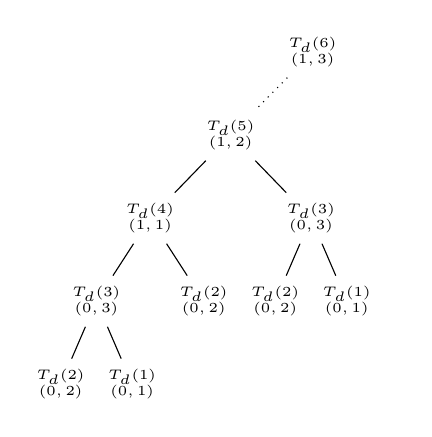
\begin{tikzpicture}
 \Tree 
	[.$T_d(6)$\\$(1,3)$ \edge[draw, dotted];
		[.$T_d(5)$\\$(1,2)$
			[.$T_d(4)$\\$(1,1)$
				[.$T_d(3)$\\$(0,3)$ $T_d(2)$\\$(0,2)$ $T_d(1)$\\$(0,1)$ ]
				$T_d(2)$\\$(0,2)$ %$T_d(1)$\\$(0,1)$
			]
			[.$T_d(3)$\\$(0,3)$ $T_d(2)$\\$(0,2)$ $T_d(1)$\\$(0,1)$ ]
			%$T_d(2)$\\$(0,2)$
		]
	\edge[draw=none]; {}
	]
\end{tikzpicture}
\end{center}
\end{frame}

\newcommand\myInvariant{
\begin{exampleblock}{Invariant}
A ball $b_v$ referenced by a node $v$ with label $(h,i)$ was placed in a bin $x$ belonging to group $i$ that, at the time of insertion of the ball $b_v$, contained at least $h+3$ other balls. 
\end{exampleblock}
}

\begin{frame}
\frametitle{Proof of activation}
\begin{block}{Lemma}
The occurrence of a bad event (i.e., a bin contains more than $L+3$ balls) implies the activation of an AWT of order $L$.
\end{block}
\bigskip
\visible<2>{
We assign balls to the nodes of the AWT s.t.:
\myInvariant
}
\end{frame}

\begin{frame}
\frametitle{Proof of activation}

\myInvariant

Let a bin contain $L+4$ balls. We assign the topmost ball to the root of the AWT:
\begin{columns}[onlytextwidth]
\begin{column}{0.5\textwidth}
\begin{center}
\begin{tikzpicture}[scale=1, edge from parent/.style=
     {draw, edge from parent path={(\tikzparentnode) -- (\tikzchildnode)}}]
\Tree 
	[.$(L,1)$ \edge[draw=black!30!red, thick];
		[.$(L-1,3)$
			[.$(L-1,2)$
				[.$(L-1,1)$ ]
				\edge[draw, densely dotted]; {}
			]
			\edge[draw, densely dotted]; {}
		]
		\edge[draw=black!30!red, thick];
		[.$(L-1,2)$ \edge[draw, densely dotted]; {} \edge[draw, densely dotted]; {} ]
	]
\end{tikzpicture}
\end{center}
\end{column}
\begin{column}{0.5\textwidth}
\begin{tikzpicture}[scale=\scalefac]
	\bab{2 4 4 2 3 4}
	\groupSep{3};
	\setNode{1}{7};
	\ball{1}{7};
	\specialBall{2}{5};
	\path (n17) edge[insert, bend left=25] (n25);
	\path (n17) edge[insert, bend left=25] (n65);
\end{tikzpicture}
\end{column}
\end{columns}
\end{frame}

\begin{frame}
\frametitle{Proof of activation}
Given a node $v$ with label $(h,i)$ that references a ball $b_v$ (which was put into some bin of group $i$ that contained at least $h+3$ other balls at the time of insertion of ball $b_v$), \alert{we conclude} that:
\begin{enumerate}
\only<1>{
\item For $1\leq j < i$, the $j$-th location of the ball $b_v$ contains at least $h+4$ balls, at the insertion time of the ball $b_v$. If it contained less balls than the $i$-th location, the Always-go-left scheme would have put the ball $b_v$ into the bin pointed to by location $j$. We assign the topmost ball in location $j$ to the child $u$ of $v$ with label $(h,j)$. 
}
\only<2>{
\item For $i < j \leq d$, the $j$-th location contains at least $h+3$ balls. If it contained less, the Always-go-left scheme would have put the ball $b_v$ into the bin location $j$ points to. We assign the topmost ball in location $j$ to the child node $u$ of $v$ labeled with $(h-1, j)$. \qed

}
\end{enumerate}
\end{frame}


\begin{frame}
\frametitle{Probability of activation}
\begin{lemma}
For any $\alpha > 0$ and large enough $L$, the activation of an AWT of order L occurs with probability at most $n^{-\alpha}$.
\end{lemma}
\medskip
\begin{itemize}
\item $k$\dots number of nodes
\item $l$\dots number of leaves
\item $\omega$\dots number of ways to assign balls to the nodes of an AWT
\item $p_\mathrm{e}$\dots probability that all edge events occur
\item $p_\mathrm{l}$\dots probability that all edge events occur
\item $P_\mathrm{a}$\dots probability of activation of an AWT of order $L$
\end{itemize}

\begin{align*}
P_\mathrm{a} = \omega p_e p_l \quad , \quad \omega = n^k 
\end{align*}
\end{frame}

\begin{frame}
\frametitle{Edge events}
\defEdgeEvent
\bigskip
One edge is activated with probability at most $d/n$ and we have $k-1$ edges; thus
\begin{align*}
p_\mathrm{e} \leq \left(\frac{d}{n}\right)^{k-1} \quad .
\end{align*}
\end{frame}

\begin{frame}
\frametitle{Leaf events}
\only<1>{
\defLeafEvent
At any time step $t$, at most $n/3$ bins contain 3 or more balls. But \alert{how are they distributed} among the $d$ groups?

\medskip
$b_i$\dots number of bins in group $i$ containing 3 or more balls
$\beta_i = b_i d/n$\dots fraction of bins $b_i$ in group $i$
}
\only<1-2>{
\begin{align*}
\frac{n}{d}\sum_{i=1}^d \beta_i \leq \frac{n}{3} \implies
\sum_{i=1}^d \beta_i \leq \frac{d}{3}
\end{align*}
}

\only<2>{
The probability that all $d$ locations of a ball point to a bin containing 3 or more balls is
\begin{align*}
p_\mathrm{l}' = \prod_{i=1}^{d} \beta_i \quad ,
\end{align*}
which is maximized when all $\beta_i$ are equal and thus
\begin{align*}
p_\mathrm{l}' \leq  \left(\frac{1}{3}\right)^d \implies p_\mathrm{l} \leq 3^{-dl} \quad .
\end{align*}
}
\end{frame}

\begin{frame}
\frametitle{Probability of activation}
Putting it together, we get
\begin{align*}
P_\mathrm{a} \leq \omega p_e p_l \leq  n^k \left(\frac{d}{n}\right)^{k-1} 3^{-dl} \quad .
\end{align*}
Using $ k\leq 2l$, $2d^2\leq 3^d$ and $l \geq \Phi_d^{dL-1}$, we can simplify to
\begin{align*}
P_\mathrm{a} \leq n 2 ^{-\Phi_d^{dL-1}} \quad .
\end{align*}
For arbitrary $\alpha > 0$, let
\begin{align*}
L &\geq \left\lceil{\frac{\ln\log_2 n + \ln\left(1+\alpha\right)}{d \ln \Phi_d}}\right\rceil+\frac{1}{d} \implies \frac{\ln\ln n}{d \ln \Phi_d} + O\left(1\right) ,
\end{align*}
and we get
\begin{align*}
P_\mathrm{a} \leq n^{-\alpha} \xqed{5cm}
\end{align*}
\end{frame}

\begin{frame}
\frametitle{The big picture}
\theoremVocking
\assumptionOne
\medskip 
Next steps:
\begin{itemize}
\item Prove \alert{without} the simplifying assumption (V\"ocking, 2003).
\item Prove for the \alert{heavily loaded} case (Berenbrink et al.,~2006).
\end{itemize}
\end{frame}

\begin{frame}
\frametitle{Conclusion}
\begin{enumerate}
\item The balls-into-bins model \alert{adopts naturally} to various problems (hashing, load balancing,\dots).
\item Applying the two-choice paradigm reduces the upper bound for the maximum load by an \alert{exponential factor} (compared to the single choice scheme).
\item \alert{Many variations} possible: Non-uniform balls/bins; weighted balls; parallel allocation of several balls;\dots
\item \alert{Witness trees} are a suitable proof technique for this kind of problems.
\end{enumerate}
\end{frame}

\begin{frame}[shrink]
\frametitle<presentation>{References}    
\bibliographystyle{acm}
\nocite{VOC03}
\nocite{ABKU99}
\nocite{RS98}
\nocite{BCSV06}
\nocite{capocelli1990generalized}
\setbeamertemplate{bibliography item}[text]
\bibliography{../sources}
\end{frame} 	


\end{document}

%  LocalWords: 
